\documentclass[12pt]{article}
\usepackage[utf8]{inputenc}
\newcommand\preamble{
    \usepackage[italian]{babel}
    \usepackage{geometry}
    \usepackage{amsmath}
    \usepackage{amssymb}
    \usepackage{graphicx}
    \usepackage{ulem}
    \usepackage[dvipsnames]{xcolor}

    \geometry{margin=2cm}
    \let\olditemize\itemize
    \renewcommand\itemize{\olditemize\setlength\itemsep{0em}}
    \graphicspath{{../Immagini/}}

    \author{Lorenzo Vaccarecci}
}
\preamble

\title{Indici ad Albero o (ordinati)}
\date{22 Marzo 2024}

\begin{document}
\maketitle
\section{Introduzione}
\begin{description}
    \item[Organizzazione primaria]: l'insieme dei file dei dati
    \item[Organizzazione secondaria]: l'insieme dei file per indici ordinati 
\end{description}
Le coppie $(k_{i},r_{i})$ vengono memorizzate in un file su disco (\textbf{organizzazione secondaria}), ordinate rispetto ai valori della chiave $k_{i}$. Se l'indice è molto piccolo, può essere tenuto in memoria principale. Altrimenti è necessario tenerlo su disco, quindi per rendere più efficiente l'accesso alle coppie dell'indice si usa una \textcolor{Cyan}{struttura multilivello}.\\
L'indice assume una \textbf{struttura ad albero} in cui ogni nodo dell'albero corrisponde a un blocco dati.
\section{Requisiti}
I requisiti fondamentali per indici di memoria secondaria
\begin{itemize}
    \item \textbf{Bilanciamento}: il cammino dalla radice a ogni blocco deve essere distante uguale;
    \item \textbf{Occupazione minima}: ogni blocco conterrà sempre un certo numero di informazioni (pieno almeno la metà, non vogliamo blocchi vuoti);
    \item \textbf{Efficienza di aggiornamento}: le operazioni di aggiornamento devono avere costo limitato.
\end{itemize}\newpage
\section{B$^{+}$-Tree}
\subsection{Caratteristiche}
\begin{itemize}
    \item Ogni nodo corrisponde a un blocco
    \item Albero bilanciato (le operazioni di ricerca, inserimento e cancellazione hanno costo, nel caso peggiore) \begin{itemize}
        \item lineare nell'altezza dell'albero $h$
        \item logaritmico: $h=O(\log n)$
    \end{itemize}
    \item il numero massimo di elementi(=coppie) memorizzabili in un nodo è $m-1$ dove $m$ mi dice quanti puntatori al massimo sono contenuti in un nodo ($m$ può essere maggiore di 2 quindi l'albero non è solo binario).
    \item Garantiscono che ogni blocco (tranne la radice) è pieno almeno al 50\% ($\lceil \frac{m}{2} \rceil-1$).
\end{itemize}
\Tree [.$B_{0}$ 
    [ .$B_{1}$\\(pl,k,pr)(pl,k,pr) $B_{3}$\\(pl,k,pr)(pl,k,pr) $B_{4}$\\(pl,k,pr)(pl,k,pr) ] 
    [ .$B_{2}$\\(pl,k,pr)(pl,k,pr) $B_{5}$\\(pl,k,pr)(pl,k,pr) $B_{6}$\\(pl,k,pr)(pl,k,pr) ]
] 
\begin{flushleft}
    Nelle parentesi ci sono i puntatori ai figli. Nel caso delle foglie i puntatori punteranno all'organizzazione primaria. I nodi foglia hanno anche i puntatori ai nodi foglia successivi come una lista. I nodi puntano ai figli in base al valore delle chiavi.
\end{flushleft}
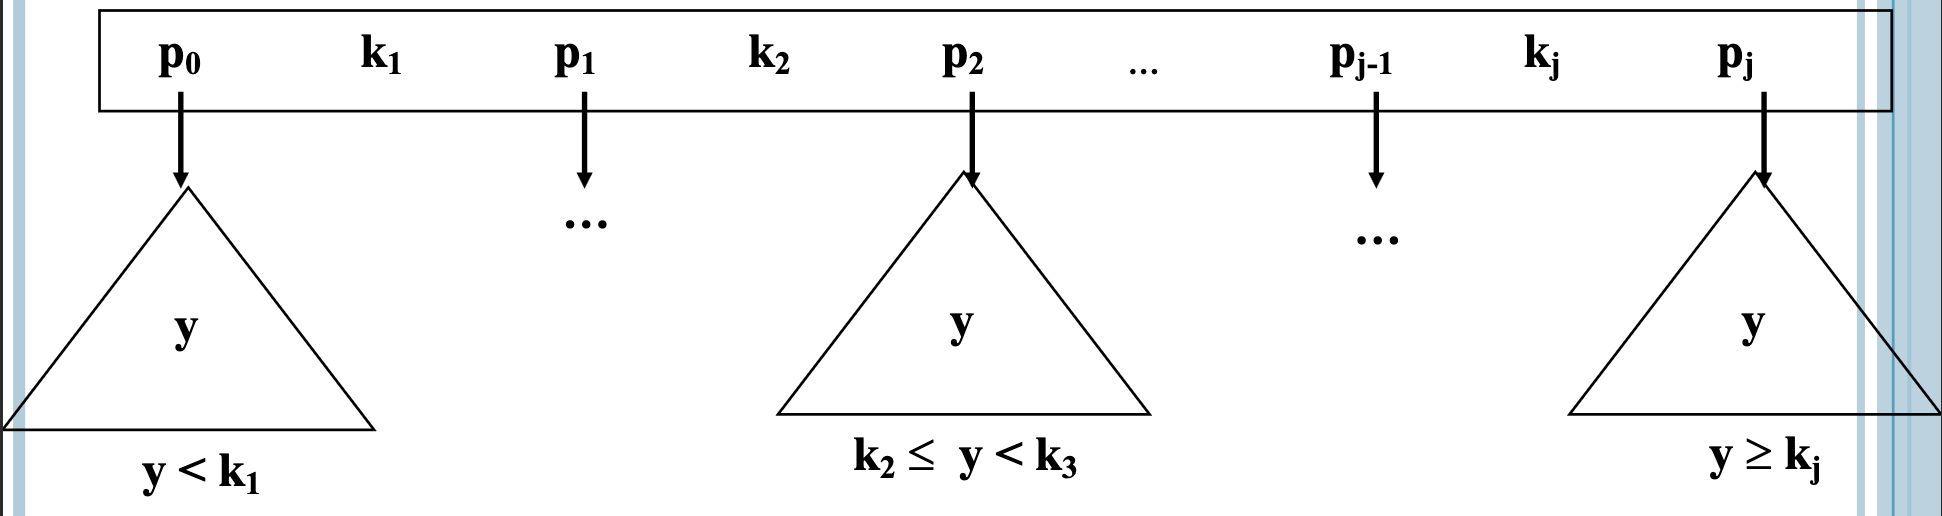
\includegraphics[width=\textwidth]{chiavialbero.png}
\textit{Il sottoalbero di sinistra di un separatore(k) contiene valori di chiave minori del separatore, quello destro maggiori o uguali}\newpage
\subsection{Ricerca}
Le ricerche possono essere effettuate per indice primario e secondario, ovviamente le foglie punteranno a strutture diverse in base al tipo di indice usato.
\subsubsection{Per uguaglianza}
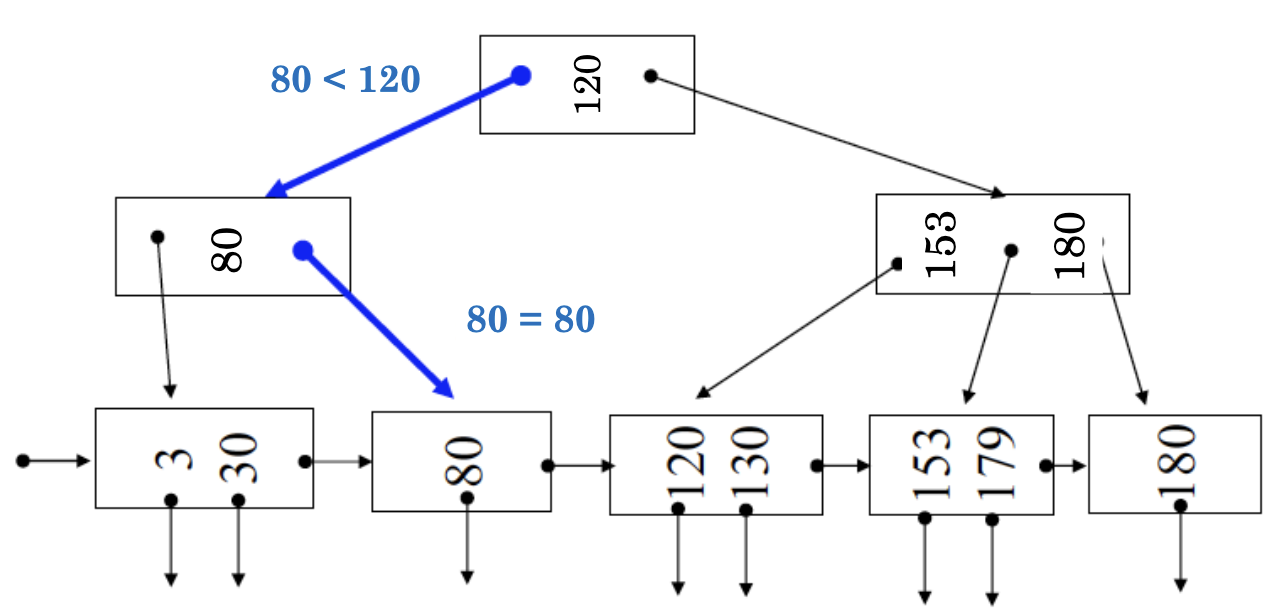
\includegraphics[width=\textwidth]{ricercaindici.png}
\begin{enumerate}
    \item La radice viene caricata nel buffer e il valore viene confrontato con il valore di ricerca ($K$) se è minore si scende a sinistra, altrimenti centrale o destra
    \item Si scende nel sottoalbero e viene controllato che il valore sia quello ricercato, se lo è scendo nel sottoalbero puntato dal numero ricercato.
    \item Ritorno al passo 1 fino a quando il nodo non punta all'organizzazione primaria. Se il valore non esiste non si accede ai file dati.
\end{enumerate}
\subsubsection{Per intervallo}
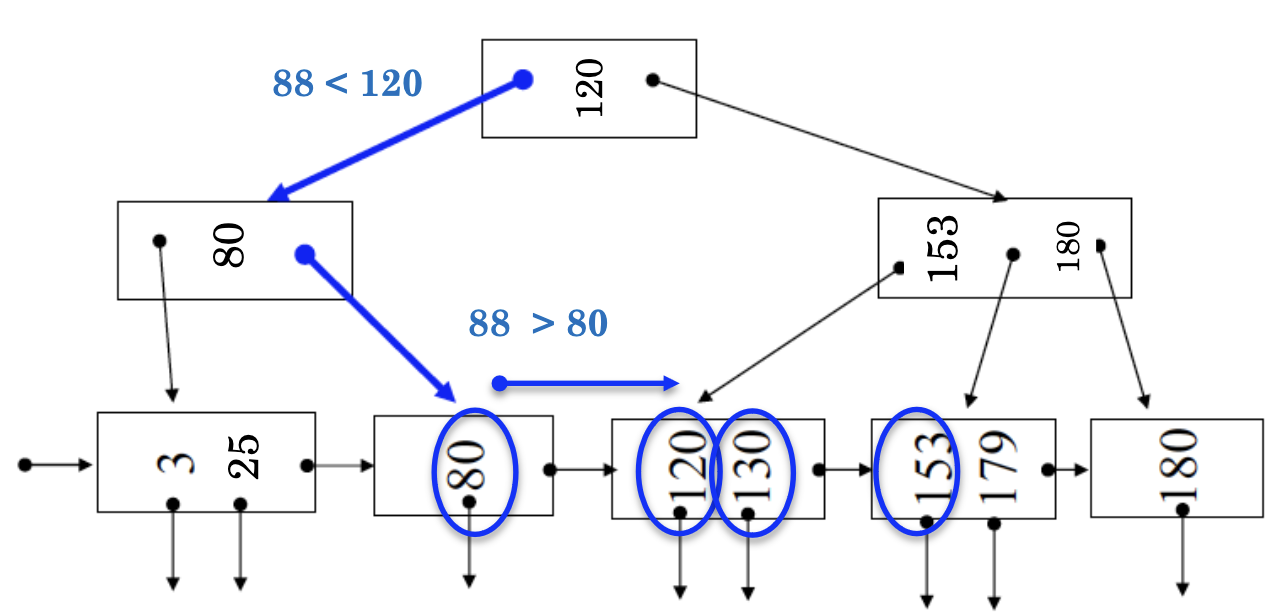
\includegraphics[width=\textwidth]{ricercaindiciintervallo.png}
Molto simile alla ricerca per uguaglianza solo che se non c'è controllo qual è la prima foglia a soddisfare la condizione (ad esempio nell'immagine il numero 88 è maggiore del numero più "vicino" quindi so che tutti i nodi a destra di quel nodo potrebbero soddisfare la condizione).
\section{Inserimento}
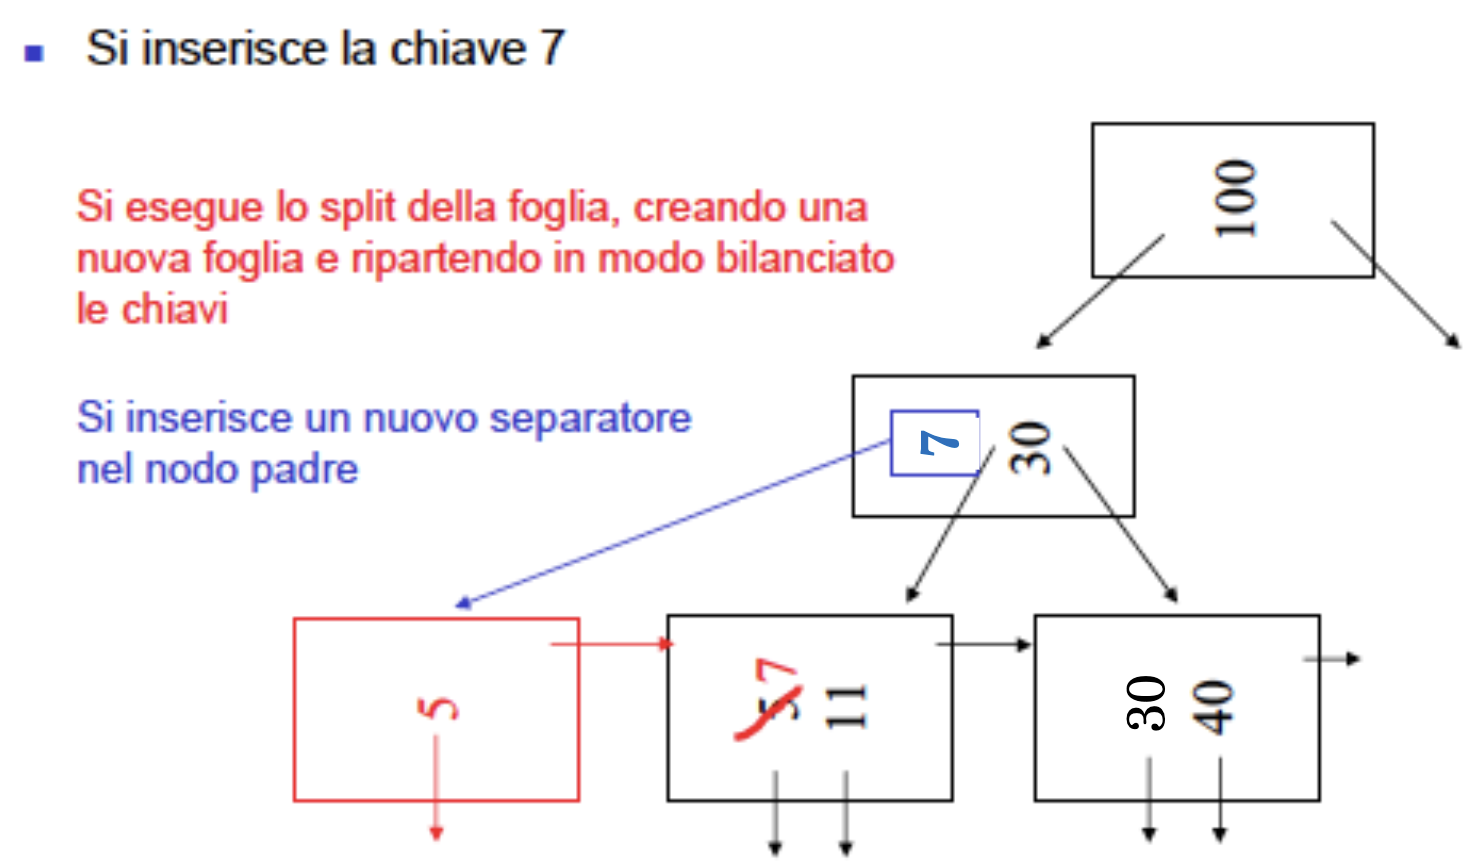
\includegraphics[width=\textwidth]{inserimento.png}
Lo split avviene nel primo nodo pieno che si incontra. Per nodo pieno si intende che non c'è spazio per inserire un nuovo separatore.
\section{Cancellazione}
Simile all'inserimento.
\end{document}